\subsection{L’émergence du web sémantique : un nouveau paradigme pour la normalisation.}

Le W3C et le développement des standards pour le web
Le web sémantique représente une nouvelle étape dans la normalisation des données. Initié par le W3C (World Wide Web Consortium), il repose sur des standards tels que RDF (Resource Description Framework) et OWL (Web Ontology Language), qui permettent de structurer les données sur le web de manière à ce qu’elles soient compréhensibles non seulement par les humains, mais aussi par les machines.\newline

Le web sémantique introduit l’idée d’un réseau de données où les informations sont liées entre elles, remplaçant ainsi les bases de données isolées.\newline

\textbf{Le web sémantique et LIDO : un lien entre les technologies et la muséographie}\newline

Dans le domaine muséal, le standard LIDO (Lightweight Information Describing Objects) a été développé pour répondre aux besoins spécifiques de description des objets de musée dans un environnement web sémantique. Ainsi le modèle LIDO permet d'intégrer des données structurées provenant de différentes sources, tout en assurant leur interopérabilité et leur lisibilité à travers des plateformes numériques. Ce standard a été conçu pour être suffisamment flexible afin de s’adapter aux diverses pratiques muséographiques : les données renseignées peuvent varier de par leur nature, leur quantités et leur précisions, d’une institution à une autre (elles peuvent aussi variées en  fonctions de qui les renseigne, un régisseur, un conservateur…). Mais il reste suffisamment rigide pour garantir une cohérence dans la structuration des données.\newline

Avec l’avènement du numérique et plus tard du web sémantique, un nouvel horizon s’est ouvert pour les institutions culturelles. Le web sémantique, introduit par Tim Berners-Lee dans les années 2000, proposait une structure où les données pouvaient être interconnectées et accessibles de manière fluide, à travers des relations sémantiques entre objets numériques. Ce modèle visait à rendre l’information non seulement accessible par l’humain, mais aussi exploitable par les machines, permettant ainsi des recherches plus intelligentes, la découverte de liens cachés entre les données, et surtout une interopérabilité accrue entre les différentes bases de données des institutions.\newline

Dans ce cadre, la science de l’information a joué un rôle central, car elle fournit les méthodes et les outils nécessaires pour organiser et structurer les masses de données générées par les musées, bibliothèques et archives. Avec son expertise dans les techniques de classification et de structuration des données, elle a pu fournir les bases théoriques et pratiques pour répondre à ces besoins de normalisation.\newline

Cependant, si ces technologies promettaient une interconnexion fluide des données, le chemin vers une adoption généralisée du web sémantique dans le secteur culturel s'est révélé plus complexe que prévu.
En effet, l’un des premiers obstacles à surmonter a été la diversité des formats de données utilisés par les institutions. Historiquement, chaque musée, chaque archive, et chaque bibliothèque avait développé ses propres méthodes et outils de gestion de l’information, en fonction de ses besoins spécifiques. Cela a conduit à une fragmentation des données et à une difficulté croissante d’interconnexion entre ces systèmes. Par exemple, les bibliothèques avaient adopté des standards comme le MARC pour la gestion de leurs collections de livres, tandis que les musées utilisaient des systèmes plus spécialisés, adaptés à la complexité de leurs objets.\newline

En outre, la montée en puissance des technologies du web sémantique a amplifié la nécessité de standardiser les données. Pour que les machines puissent comprendre et exploiter les informations, il est impératif que celles-ci soient structurées de manière cohérente. \newline
Le web sémantique introduit des concepts clés comme le Resource Description Framework (RDF), recommandé par le W3C en 1999, qui permet de représenter les données sous forme de triplets (sujet, prédicat, objet, par exemple "La Joconde - a pour peintre - Léonard De Vinci), et des ontologies, qui définissent les relations entre ces différents éléments.\footcite{rdf_champin}

\begin{figure}[h!]
	\centerline{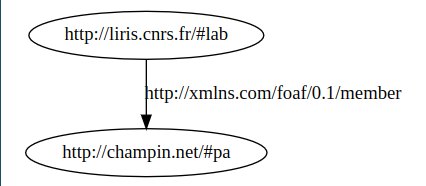
\includegraphics[width=\textwidth] {medias/schema_rdf.png}}
	\caption{Exemple de triplet en RDF}
\end{figure}

Ces innovations ont permis de poser les bases d’une interopérabilité sémantique, où des systèmes différents peuvent échanger et comprendre des données dans un langage commun.\newline

Malgré les avancées théoriques, la mise en pratique de ces concepts a rencontré plusieurs défis. D’une part, le coût élevé des technologies associées au web sémantique a freiné l’adoption de ces outils, en particulier dans les institutions culturelles disposant de ressources limitées. D’autre part, les compétences techniques nécessaires pour implémenter ces solutions ont également constitué un obstacle majeur. Les musées, en particulier, ont dû relever un défi supplémentaire : celui de l’adaptation des standards globaux aux réalités locales de leurs collections et de leurs pratiques. \newline

Ainsi, la science de l’information a progressivement évolué pour répondre à ces nouveaux défis numériques, mais elle a également montré ses limites. Le besoin de solutions pragmatiques et adaptées aux contextes variés des institutions culturelles a conduit à l’émergence de modèles spécifiques, comme LIDO ou CIDOC CRM, qui seront explorés plus en détail dans les parties suivantes. Ces modèles visent à combler l’écart entre la théorie et la pratique, en offrant des solutions de normalisation qui prennent en compte la diversité des collections et des pratiques des musées.\newline

\textbf{Les promesses et les limites des technologies du web sémantique dans les institutions culturelles}\newline

Le web sémantique a apporté de nombreuses promesses aux institutions culturelles, notamment en facilitant l’interconnexion des données à travers des systèmes disparates. En théorie, cette technologie permet de surmonter les barrières qui séparaient autrefois les différentes institutions et leurs bases de données, en créant un réseau sémantique où chaque objet numérique est relié à d’autres informations, qu’elles soient locales ou externes à l’institution.\newline

L’une des principales forces du web sémantique réside dans sa capacité à connecter les données en utilisant des formats normalisés et des ontologies communes. Par exemple, une œuvre d’art numérisée dans un musée peut être liée à des informations biographiques sur l’artiste, disponibles dans une autre base de données. Ce type de connexion transversale permet non seulement de donner plus de contexte à chaque objet, mais aussi de faciliter des recherches plus complexes, où les utilisateurs peuvent naviguer d’une œuvre à une autre en suivant des liens sémantiques.\newline

Un autre avantage clé du web sémantique est la possibilité d'automatiser certaines tâches de recherche et d'organisation des données. Grâce à des technologies comme le SPARQL, il est possible d'interroger des bases de données en réseau et d’obtenir des résultats qui combinent des informations provenant de différentes sources. Cela ouvre la voie à des recherches plus puissantes et à des découvertes qui auraient été impossibles dans un cadre plus cloisonné. Pour les musées, cela signifie une opportunité de mieux valoriser leurs collections, en les rendant plus accessibles et plus interconnectées avec d'autres institutions. \newline

Toutefois, malgré ces avantages théoriques, l’adoption du web sémantique dans les institutions culturelles a été ralentie par plusieurs facteurs. Tout d’abord, la complexité technique des technologies associées au web sémantique a constitué un obstacle majeur. Pour implémenter des systèmes basés sur des ontologies et des modèles sémantiques, les musées doivent disposer de compétences techniques spécifiques, souvent coûteuses. De nombreuses institutions, en particulier les plus petites, n’ont ni les ressources humaines ni les moyens financiers pour adopter ces technologies à grande échelle.\newline

De plus, la diversité des collections et des pratiques entre les institutions culturelles pose un défi supplémentaire. Chaque musée possède ses propres particularités, ses propres systèmes de gestion, et souvent des méthodes d’indexation et de description qui varient considérablement d’un établissement à l’autre. Cette diversité rend difficile l’adoption d’un modèle universel qui conviendrait à toutes les institutions. Même avec des modèles normalisés comme LIDO ou CIDOC CRM, chaque musée doit adapter le modèle à ses propres besoins, ce qui complique l’interopérabilité.
Enfin, l'une des limites inhérentes du web sémantique est qu'il repose sur la qualité des données qui sont intégrées dans le système. Si les données sont mal structurées, incomplètes ou obsolètes, même les meilleures technologies ne peuvent produire des résultats satisfaisants. La qualité des métadonnées devient donc un enjeu crucial pour garantir le succès des projets de web sémantique dans les musées.\newline

Le décalage entre les promesses initiales du web sémantique et la réalité de son adoption dans les musées nous conduit à une réflexion plus large sur la manière dont ces technologies peuvent être adaptées aux besoins des institutions culturelles. Il est clair que si le web sémantique offre des possibilités immenses, il doit être accompagné de processus de normalisation rigoureux, mais aussi de solutions adaptées aux réalités pratiques et économiques des musées. Cela nécessite une coopération étroite entre les développeurs de technologies, les experts en gestion de collections, et les décideurs culturels.

